\documentclass[10pt, technote, oribibl, unicode]{beamer}
\usepackage[english]{babel}
\usepackage[utf8x]{inputenc}
\usepackage[T1]{fontenc}
\usepackage{bbding}
\usepackage{animate}
\usepackage{xcolor}
\usepackage{color}
\usepackage{colortbl}
% include file and not recompile it
\usepackage{standalone}
\usepackage{dsfont}

\usepackage{numprint}
\npthousandsep{\,}
\newcommand{\quotes}[1]{``#1''}


\usetheme{unibo}

\title{Implementation and optimization of algorithms in Biomedical Big Data Analytics}
\subtitle{PhD Thesis discussion}
\date[March 16, 2020]{March 16, 2020}
\author[Nico Curti]{Nico Curti}
\supervisor{Prof. Daniel Remondini}
\cosupervisor{Prof. Gastone Castellani\\Prof. Armando Bazzani}


\begin{document}

\begin{frame}

  \titlepage

\end{frame}


\begin{frame}{Purposes}{Biomedical Big Data Analytics}

  \begin{columns}

    \begin{column}{0.5\textwidth}

      \begin{exampleblock}{Feature Selection\\DNetPRO}
        \begin{itemize}
          \item[$\diamond$] \textbf{Topic:} Gene Expression Analysis;

          \item[$\diamond$] \textbf{Characteristics:} Novel algorithm \& optimization on distributed computing;

          \item[$\diamond$] \textbf{Applications:}
            \begin{itemize}
              \item Synthetic dataset;
              \item Benchmark TCGA datasets;
              \item Cytokinoma;
              \item Bovine Signature;
              \item Pedestrian mobility in Venice;
            \end{itemize}

          \item[$\diamond$] \textbf{URL:} \url{https://github.com/Nico-Curti/DNetPRO};
        \end{itemize}
      \end{exampleblock}

    \end{column}
    \begin{column}{0.5\textwidth}

      \begin{block}{Deep Learning\\Byron}
        \begin{itemize}
          \item[$\diamond$] \textbf{Topic:} Neural Network models;

          \item[$\diamond$] \textbf{Characteristics:} Code Optimization and multi-threading parallelization;

          \item[$\diamond$] \textbf{Applications:}
            \begin{itemize}
              \item Super Resolution;
              \item Object Detection;
              \item Image Segmentation;
            \end{itemize}

          \item[$\diamond$] \textbf{URL:}
            \begin{itemize}
              \item \tiny{\url{https://github.com/Nico-Curti/NumPyNet};}
              \item \tiny{\url{https://github.com/Nico-Curti/Byron};}
            \end{itemize}
        \end{itemize}
      \end{block}

    \end{column}

  \end{columns}

  \begin{alertblock}{Big Data\\CHIMeRA}
    \begin{columns}
      \begin{column}{0.45\textwidth}
        \begin{itemize}
          \item[$\diamond$] \textbf{Topic:}
            \begin{itemize}
              \item Biomedical Big Data;
              \item Database service;
              \item Network analysis;
              \item Natural Language Processing;
              \item Web scraping;
              \item Data harmonization;
            \end{itemize}
          \end{itemize}
      \end{column}
      \begin{column}{0.55\textwidth}
        \begin{itemize}
          \item[$\diamond$] \textbf{Characteristics:} Merging of public available knowledge into network structure;
          \item[$\diamond$] \textbf{Applications:} Leukemia;
          \item[$\diamond$] \textbf{URL:} Not available yet;
        \end{itemize}
      \end{column}
    \end{columns}
  \end{alertblock}

\end{frame}



\documentclass{standalone}

\begin{document}

\setbeamerfont{block body}{size=\scriptsize}
\setbeamerfont{block body example}{size=\scriptsize}
\setbeamerfont{block body alerted}{size=\scriptsize}
\setbeamertemplate{itemize/enumerate body begin}{\scriptsize}
\setbeamertemplate{itemize/enumerate subbody begin}{\scriptsize}

\begin{frame}{The Big Data era}{Biological Big Data}

  \setbeamercolor{block title example}{bg=white, fg=DarkGreen}
  \setbeamercolor{block body example}{bg=white, fg=black}

  \scriptsize{Considering the annual growth of data generation, the digital universe (i.e. data we generate annually) will reach 44 zettabytes by the year 2020, which is ten times the size of the digital universe in 2013. This trend in rising data volume is supported by:}

  \begin{figure}
    \centering
    \includegraphics[width=.5\linewidth]{grow.jpg}
  \end{figure}

  \begin{exampleblock}{Single Sequenced Human Genome}
    The size of a single sequenced human genome is approximately 200 Gb for less than US \$ \numprint{1000} (National Human Genome Research Institute, 2016).
  \end{exampleblock}

  \begin{exampleblock}{Datasets available online}
    The amount of available data from large project such as \numprint{1000} Genomes (\url{http://www.1000genomes.org}) will collectively approach the petabyte scale for the raw information alone.
  \end{exampleblock}

\end{frame}



\begin{frame}{A new research paradigm}{Biological Big Data}

  \setbeamertemplate{itemize items}[ball]

  \begin{columns}

    \begin{column}{0.5\textwidth}

      The problems concerning the Big Data Analytics must be faced on two fronts:

      \vspace{0.6cm}
      \textbf{Algorithm and Models:}

      \begin{itemize}

        \item Data visualization
        \item Dimensionality reduction
        \item Parallel computing
        \item Optimization

      \end{itemize}

    \end{column}
    \begin{column}{0.5\textwidth}

      \begin{figure}
        \centering
        \includegraphics[width=.8\linewidth]{h2020.jpg}
      \end{figure}

      \textbf{Hardware and Technology:}

      \begin{itemize}

        \item HPC
        \item Cloud
        \item Storage
        \item Data exchange

      \end{itemize}

    \end{column}
  \end{columns}

  \vspace{0.5cm}

  A \textbf{new paradigm} is emerging and it needs new hybrid sciences as Bioinformatics, Computational Sociology and new hybrid tools as Hybrid Cloud Architecture, Data Mining Algorithms.

\end{frame}


\begin{frame}{Biological features}{Gene expression Big Data}

  \setbeamertemplate{itemize items}[ball]

  \begin{columns}

    \begin{column}{0.4\linewidth}

      \begin{figure}[htbp]
        \centering
        \def\svgwidth{0.8\linewidth}
        \input{./img/distributions.pdf_tex}
      \end{figure}

    \end{column}
    \begin{column}{0.6\linewidth}

      \begin{itemize}
        \item single parameter classification fails in predicting higher dimension classification performance;

        \item feature1 and feature2 classify badly in 1D, but have a very good performance in 2D;

        \item Activity of a biological feature as a function of its expression level: monotonically increasing; "windowed" behavior.

      \end{itemize}

    \end{column}
  \end{columns}

  \begin{figure}[htbp]
    \centering
    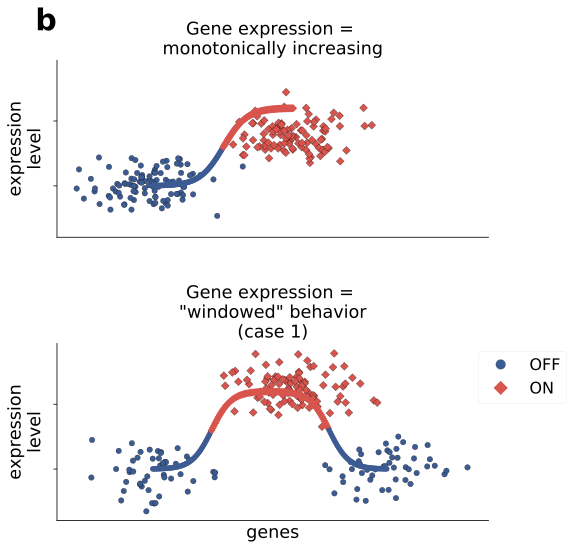
\includegraphics[width=0.9\linewidth]{expression.png}
  \end{figure}

\end{frame}


\begin{frame}{Classification and dimensionality reduction}{DNetPRO algorithm}

  \setbeamertemplate{itemize items}[ball]

  The potential clinical utility of genomic, transciptomic, epigenomic and proteomic data in aggregate remains largely unknown.

  The goal of these type of analyses is to identify the \textbf{smallest number of probes} able to hold the most information about classes.

  \vspace{.5cm}

  \textbf{DNetPRO} (Discriminant analysis with Network PROcessing) algorithm:

  \vspace{1cm}

  \begin{columns}

    \begin{column}{0.5\linewidth}

      \textbf{Computational Field:}

      \begin{itemize}
        \item Feature selection
        \item Dimensionality reduction
        \item Classification
      \end{itemize}

    \end{column}

    \begin{column}{0.5\linewidth}

      \textbf{Biological Field:}

      \begin{itemize}
        \item Evaluation of genes interaction
        \item Easy interpretation
        \item Extraction of Signature
      \end{itemize}

    \end{column}

  \end{columns}

\end{frame}

%% OPTIMIZATIONS

\begin{frame}{DNetPRO algorithm}{Pipeline description}

  \begin{figure}
    \begin{overprint}
      \onslide<1>\centering\includegraphics[width=0.8\linewidth]{pseudo_dnet.png}
      \onslide<2>\vspace{1cm}\centering\includegraphics[width=\linewidth]{dnet_pipe.png}
    \end{overprint}
  \end{figure}

\end{frame}


\begin{frame}{DNetPRO algorithm}{Algorithm optimization}

  Porting on a parallel environment: \textsf{C++} multi-threading implementation for network construction.

  Distributed computation of each pipeline step (\textsf{snakemake}).

  \begin{columns}

    \begin{column}{0.5\linewidth}

      \begin{figure}[htbp]
        \centering
        \def\svgwidth{0.8\linewidth}
        \input{./img/samples_timing.pdf_tex}
      \end{figure}

    \end{column}

    \begin{column}{0.5\linewidth}

      \begin{figure}[htbp]
        \centering
        \def\svgwidth{0.8\linewidth}
        \input{./img/features_timing.pdf_tex}
      \end{figure}

    \end{column}

  \end{columns}

    \begin{figure}[htbp]
      \centering
      \def\svgwidth{0.5\linewidth}
      \input{./img/nth_timing.pdf_tex}
    \end{figure}

\end{frame}

\begin{frame}{DNetPRO algorithm}{Algorithm optimization}

  Porting on a parallel environment: \textsf{C++} multi-threading implementation for network construction.

  Distributed computation of each pipeline step (\textsf{snakemake}).

  \begin{figure}
    \centering
    \includegraphics[width=\linewidth]{qdanet_pipe_single.png}
  \end{figure}

\end{frame}

%% APPLICATIONS

\begin{frame}{DNetPRO algorithm}{Applications}

  \setbeamertemplate{itemize items}[ball]

  \begin{columns}

    \begin{column}{0.5\textwidth}

      \begin{exampleblock}{Synthetic dataset}
          Study of the characteristics of the algorithm with different number of samples and features.

          \begin{figure}
            \centering
            \def\svgwidth{0.8\linewidth}
            \input{./img/features_toy.pdf_tex}
          \end{figure}

      \end{exampleblock}

    \end{column}
    \begin{column}{0.5\textwidth}

      \begin{block}{Cytokinome dataset}
        \begin{itemize}
          \item Study on Alzheimer's disease;
          \item 26 cytokine expression levels;
          \item 289 subjects (189 female and 100 male);
        \end{itemize}
      \end{block}

      \begin{alertblock}{Bovine dataset}
        \begin{itemize}
          \item Study on Paratuberculosis disease;
          \item 15 mRNA samples of 3 bovine classes;
          \item 13529 features each;
        \end{itemize}
      \end{alertblock}

    \end{column}

  \end{columns}

  \setbeamercolor{block title alerted}{fg=black, bg=orange!40!white}
  \setbeamercolor{block body alerted}{fg=black, bg=orange!20!white}

  \begin{alertblock}{Benchmark state-of-art}

    \begin{columns}
      \begin{column}{0.4\linewidth}

        \begin{itemize}
          \item Application on Synapse dataset;
          \item mRNA, miRNA and RPPA samples;
        \end{itemize}

      \end{column}
      \begin{column}{0.6\linewidth}

        \begin{itemize}
          \item 4 different tumors\\(KIRC, GBM, LUSC and OV);
          \item benchmark on state-of-art\\(Yuan et al., \emph{Nature methods}, 2014);
        \end{itemize}
      \end{column}
    \end{columns}

  \end{alertblock}

\end{frame}




\begin{frame}{Synapse dataset}{DNetPRO benchmark}

  \setbeamertemplate{itemize items}[ball]

  \begin{columns}

    \begin{column}{0.5\linewidth}
      \textbf{TCGA} dataset - The Cancer Genome Atlas

      \vspace{0.5cm}

      \textbf{Dichotomization:} normal/tumor
    \end{column}

    \begin{column}{0.5\linewidth}
      \begin{figure}
        \centering
        \includegraphics[width=\linewidth]{synapse_table.png}
      \end{figure}
    \end{column}

  \end{columns}

  \vspace{1cm}

  \begin{columns}

    \begin{column}{0.6\linewidth}

    4 cancer types:

    \begin{itemize}
      \item KIRC (\emph{Kidney Renal clear cell Carcinoma})
      \item GBM (\emph{Glioblastoma Multiforme})
      \item LUSC (\emph{Lung Squamous Cell Carcinoma})
      \item OV (\emph{Ovarian serous cystadenocarcinoma})
    \end{itemize}

    \end{column}

    \begin{column}{0.4\linewidth}

      3 molecular data types:

      \begin{itemize}
        \item mRNA
        \item miRNA (\emph{micro RNA})
        \item RPPA (\emph{Reverse Phase Protein Array})
      \end{itemize}

    \end{column}

  \end{columns}

\end{frame}




\begin{frame}{Synapse dataset}{mRNA Results}

  \scriptsize{Benchmark with 8 classifiers with different features selection methods: \textbf{DDA} (diagonal discriminant analysis); \textbf{KNN} (K-nearest neighbor); \textbf{DA} (discriminant analysis); \textbf{LR} (logistic regression); \textbf{NC} (nearest centroid); \textbf{PLS} (partial least squares); \textbf{RF} (random forest); \textbf{SVM} (support vector machine).}

  \begin{figure}
    \begin{overprint}
      \onslide<1>\centering\includegraphics[width=0.6\linewidth]{mRNA_boxplot.png}
      \onslide<2>\centering\def\svgwidth{0.7\linewidth}\input{./img/mRNA_tables.pdf_tex}
    \end{overprint}
  \end{figure}

\end{frame}


\begin{frame}{Synapse dataset}{miRNA - RPPA Results}

  \scriptsize{Benchmark with 8 classifiers with different features selection methods: \textbf{DDA} (diagonal discriminant analysis); \textbf{KNN} (K-nearest neighbor); \textbf{DA} (discriminant analysis); \textbf{LR} (logistic regression); \textbf{NC} (nearest centroid); \textbf{PLS} (partial least squares); \textbf{RF} (random forest); \textbf{SVM} (support vector machine).}

  \begin{columns}

    \begin{column}{0.5\linewidth}

      \begin{figure}
        \begin{overprint}
          \onslide<1>\centering\includegraphics[width=\linewidth]{miRNA_boxplot.png}
          \onslide<2>\centering\def\svgwidth{\linewidth}\input{./img/miRNA_tables.pdf_tex}
        \end{overprint}
      \end{figure}

    \end{column}

    \begin{column}{0.5\linewidth}

      \begin{figure}
        \begin{overprint}
          \onslide<1>\centering\includegraphics[width=\linewidth]{RPPA_boxplot.png}
          \onslide<2>\centering\def\svgwidth{\linewidth}\input{./img/RPPA_tables.pdf_tex}
        \end{overprint}
      \end{figure}

    \end{column}

  \end{columns}

\end{frame}



\begin{frame}{Cytokinome dataset}{DNetPRO Applications}

  \setbeamertemplate{itemize items}[ball]

  \begin{columns}

    \begin{column}{0.5\linewidth}

      \begin{itemize}
        \item Alzheimer's disease data.
        \item \numprint{26} number of cytokines.
      \end{itemize}

    \end{column}

    \begin{column}{0.5\linewidth}

      \begin{itemize}
        \item 3 classes: CTL (control), MCI (transient), AD (positive).
        \item 289 old-age subjects.
      \end{itemize}

    \end{column}

  \end{columns}

  \begin{figure}
    \centering
    \includegraphics[width=0.3\linewidth]{best_ctl_ad.png}
  \end{figure}

  \scriptsize{We extract the signature using the MCI class as AD-like samples.}

  \begin{figure}
    \centering
    \includegraphics[width=\linewidth]{cytokine_table.png}
  \end{figure}

\end{frame}


\begin{frame}{Cytokinome dataset}{DNetPRO Applications}

  \setbeamertemplate{itemize items}[ball]

  \scriptsize{We extract the signature using the MCI class as AD-like samples.}

  \scriptsize{Stratification according to the sex.}

  \scriptsize{We observed a different behavior between \textbf{males} (A) and \textbf{females} (B) in CTL samples.}

  \begin{columns}

    \begin{column}{0.5\linewidth}
      \begin{figure}
        \centering
        \includegraphics[width=\linewidth]{males.png}
      \end{figure}
    \end{column}

    \begin{column}{0.5\linewidth}
      \begin{figure}
        \centering
        \includegraphics[width=\linewidth]{females.png}
      \end{figure}
    \end{column}

  \end{columns}

\end{frame}


%% BOVINE

\begin{frame}{Bovine dataset}{DNetPRO Applications}

  \setbeamertemplate{itemize items}[ball]

  \begin{columns}

    \begin{column}{0.5\linewidth}

      \begin{itemize}
        \item Mycobatcterium avium subsp. paratuberculosis data.
        \item \numprint{15036} number of genes.
      \end{itemize}

    \end{column}

    \begin{column}{0.5\linewidth}

      \begin{itemize}
        \item 3 classes: NN (negative), NP (exposed), PP (positive).
        \item 15 samples per probe.
      \end{itemize}

    \end{column}

  \end{columns}

  \begin{figure}
    \centering
    \def\svgwidth{0.9\linewidth}
    \input{./img/Bovine_expression_level.pdf_tex}
  \end{figure}

\end{frame}


\begin{frame}{Bovine dataset}{DNetPRO Applications}

  \setbeamertemplate{itemize items}[ball]

  \scriptsize{We extract the signature using the PP class as NP-like samples.}

  \begin{columns}

    \begin{column}{0.4\linewidth}

      \scriptsize{\textbf{Results:}}

      \begin{itemize}
        \item Top performing signature (123 probes)
        \item Average performance 90\%
        \item Matthews Correlation Coefficient 0.82
      \end{itemize}

      \vspace{0.5cm}

      \scriptsize{\textbf{Pendant node remotion:}}

      \begin{itemize}
        \item Top performing signature (10 probes)
        \item Average performance 100\%
        \item Matthews Correlation Coefficient 1.00
      \end{itemize}

    \end{column}

    \begin{column}{0.6\linewidth}

      \begin{figure}
        \centering
        \includegraphics[width=0.75\linewidth]{Bovine_signature.png}
      \end{figure}

    \end{column}

  \end{columns}

\end{frame}


%% VENICE


\begin{frame}{Social Application}{Network pedestrian mobility}

  \setbeamertemplate{itemize items}[ball]

  \begin{columns}
    \begin{column}{0.6\linewidth}

      During major events the behavior of the crowd can lead to mobility and/or security issues.

      ICT allows for the collection of a huge number of geolocalized timestamped data which can be analysed for:

      \vspace{0.5cm}

      \begin{itemize}

        \item Crowd behavior detection and management
        \item Crowd mobility reconstruction and prediction

      \end{itemize}

      Data are provided within the Geosynthesis framework in collaboration with TIM Spa and Nokia.

    \end{column}

    \begin{column}{0.4\linewidth}
      \begin{figure}
        \centering
        \includegraphics[width=\linewidth]{venice1.png}
      \end{figure}
      \begin{figure}
        \centering
        \includegraphics[width=\linewidth]{venice2.png}
      \end{figure}

    \end{column}

  \end{columns}

\end{frame}



\begin{frame}{Social Application}{Network pedestrian mobility}

  \setbeamertemplate{itemize items}[ball]

  \begin{columns}

    \begin{column}{0.5\linewidth}

      \scriptsize{Typical dataset size : $10^6$ records/day}

      \scriptsize{Typical users number : \numprint{5000} users/day}

      \vspace{.5cm}

      \scriptsize{Acquisition periods}

      \begin{itemize}
        \item Carnevale from 23/02/2017 to 02/03/2017
        \item Festa del Redentore 14,15,16/07/2017
      \end{itemize}

    \end{column}

    \begin{column}{0.5\linewidth}

      \scriptsize{Nationality disaggregation preferred paths:}

      \begin{itemize}
        \item Italians (red, purple)
        \item Foreigners (yellow, green)
      \end{itemize}

    \end{column}

  \end{columns}

  \begin{columns}

  \begin{column}{0.4\linewidth}

    Statistics:

    \begin{itemize}
      \item Total lines : \numprint{11596039}
      \item Errors : \numprint{92713} (0.8\%)
      \item Not georef : \numprint{8715928} (75.2\%)
      \item Out of ROI : \numprint{1773013} (15.3\%)
      \item Valid : \numprint{1014385} (8.7\%)
    \end{itemize}

  \end{column}

  \begin{column}{0.6\linewidth}
    \begin{figure}
      \centering
      \includegraphics[width=\linewidth]{venice3.png}
    \end{figure}
  \end{column}

\end{columns}

\end{frame}



\begin{frame}{Social Application}{Network pedestrian mobility}

  \begin{columns}

    \begin{column}{0.5\linewidth}

      Festa del Redentore 15/07/2017

      \begin{figure}
        \centering
        \includegraphics[width=\linewidth]{redentore.png}
      \end{figure}

      Road network length fraction : 13\%
      Mobility explained : 65\%


    \end{column}

    \begin{column}{0.5\linewidth}

      Carnevale 26/02/2017

      \begin{figure}
        \centering
        \includegraphics[width=\linewidth]{carnival.png}
      \end{figure}

      Road network length fraction : 15\%
      Mobility explained : 64\%

    \end{column}

  \end{columns}

\end{frame}


\begin{frame}{Conclusion}{DNetPRO Algorithm Applications}

  \setbeamertemplate{itemize items}[ball]

  \begin{itemize}

    \item We proposed a novel technique of feature selection based on graph analysis;

    \item The method is optimized from a computational point of view and a it represents a valid alternative to standard methods;

    \item We proved the efficiency of DNetPRO algorithm on synthetic data proving its pros and cons;

    \item We highlighted its efficiency also in relation to state-of-art results on gene expression data;

    \item We applied the DNetPRO on several (real) dataset obtaining interesting results in several topics;

    \item We generalize the application of the DNetPRO algorithm also in non-biological data;

  \end{itemize}

\end{frame}


\end{document}

\documentclass{standalone}

\begin{document}

\setbeamerfont{block body}{size=\scriptsize}
\setbeamerfont{block body example}{size=\scriptsize}
\setbeamerfont{block body alerted}{size=\scriptsize}
\setbeamertemplate{itemize/enumerate body begin}{\scriptsize}
\setbeamertemplate{itemize/enumerate subbody begin}{\scriptsize}

\begin{frame}{Deep Learning}{Neural Network models}

  \setbeamertemplate{itemize items}[ball]

  \scriptsize{Deep Learning model is becoming equivalent to Neural Network architecture/model, i.e a more or less complex pipeline of functions which takes in input a sample and it applies a series of transformations to obtain the desired result.}

  \begin{block}{Objectives}
    \begin{itemize}

      \item Optimization and extension of state-of-art Neural Network libraries;

      \item  Development of two novel libraries, for education and analytic purposes, respectively;

      \item Improve parallelization strategies to reach the best computational performances in cluster machine without GPUs supports;

    \end{itemize}

  \end{block}

  \begin{alertblock}{}
    All the algorithm and codes developed are \textbf{tested}, \textbf{documented} and \textbf{public available}!

    \quad

    \textbf{Reference:} \url{https://nico-curti2.gitbook.io/phd-thesis} (GitBook documentation).
  \end{alertblock}

\end{frame}


\setbeamertemplate{itemize/enumerate body begin}{\footnotesize}
\setbeamertemplate{itemize/enumerate subbody begin}{\footnotesize}

\begin{frame}{What is a Deep Learning model?}{Neural Network models}
  \setbeamertemplate{itemize items}[ball]

  \begin{itemize}
    \item Neural Networks are mathematical models \textbf{commonly used} in data analysis.

    \item From a theoretical point-of-view we can define a Neural Network as \textbf{a series of non-linear multi-parametric functions}.

    \item Neural Networks are considered as \textbf{Universal Function Approximators}.
  \end{itemize}

  \begin{figure}[hbp]
    \centering
    \includegraphics[width=0.85\textwidth]{net_scheme.png}
    \caption{\scriptsize{Neural Network model scheme.
             The model is composed by a series of layers made by interconnected computational units.
             The connections between layers can be serials or parallels and each layer models a pre-determined mathematical function.
             %The model parameters are tuned during the training procedure, i.e the model is fed with a series of labeled examples and its efficiency can be evaluated on new (test) data.
            }}
  \end{figure}

\end{frame}

\begin{frame}{State-of-art libraries}{Why other two libraries?}

  \scriptsize{A wide range of documentations and implementations have been written on Deep Learning and it is more and more hard to move around the different sources.}

  \scriptsize{Leader on this topic are became the multiple open-source `Python` libraries available on-line as \href{http://tensorflow.org}{Tensorflow}, \href{http://pytorch.org}{Pytorch} and \href{http://doi.acm.org/10.1145/2647868.2654889}{Caffe}.}

  \begin{columns}

    \begin{column}{0.5\textwidth}

      \begin{block}{Pros}
        \begin{itemize}
          \item[$\diamond$] Simplicity in writing complex models in a minimum number of code lines;
          \item[$\diamond$] Simplicity of the \textsf{Python} language;
          \item[$\diamond$] Extremely efficient in GPU environments;
        \end{itemize}
      \end{block}
    \end{column}
    \begin{column}{0.5\textwidth}

      \begin{alertblock}{Cons}
        \begin{itemize}
          \item[$\diamond$] Steep learning curve for complex applications or algorithm modifications;
          \item[$\diamond$] Hard to manage as services;
          \item[$\diamond$] They are not designed for CPU performances;
        \end{itemize}
      \end{alertblock}
    \end{column}

  \end{columns}

  \vspace{0.5cm}

  \scriptsize{Only a small part of the research community uses more deeper implementation in \textsf{C++} or other low-level programming languages.}
  \scriptsize{About them it should be mentioned the \textsf{darknet project} of Redmon J. et al. which created a sort of standard in object detection applications using a pure \textsf{Ansi-C} library.}

\end{frame}

\begin{frame}{NumPyNet \& Byron}{Why other two libraries?}

  \setbeamercolor{block title alerted}{fg=black, bg=orange!40!white}
  \setbeamercolor{block body alerted}{fg=black, bg=orange!20!white}

  \setbeamertemplate{itemize/enumerate body begin}{\tiny}
  \setbeamertemplate{itemize/enumerate subbody begin}{\tiny}

  \setbeamertemplate{itemize items}[ball]

  \begin{columns}

    \begin{column}{0.5\textwidth}
      \begin{block}{NumPyNet \hfill\includegraphics[width=.1\textwidth]{python.png}}
        \begin{itemize}
          \item \textbf{LANGUAGE:} \textsf{Python};
          \item \textbf{INSTALLATION:} \textsf{Setup} (\textsf{PyPI} upload wip);
          \item \textbf{OS:} Linux \& MacOS \& Windows;
          \item \textbf{DOCUMENTATION:} fully documented;
          \item \textbf{PURPOSE:} educational / study;
          \item \textbf{CI:} Travis \& Appveyor;
          \item \textbf{USAGE:} model design / algorithm improvements;
          \item \textbf{MISCELLANEOUS:} all functionality are tested against \textsf{Keras} counterpart;
          \item \textbf{URL:} \url{https://github.com/Nico-Curti/NumPyNet}
        \end{itemize}
      \end{block}
    \end{column}
    \begin{column}{0.5\textwidth}
      \begin{alertblock}{Byron \hfill\includegraphics[width=.1\textwidth]{cpp.png}}
        \begin{itemize}
          \item \textbf{LANGUAGE:} \textsf{C++} Standard 17;
          \item \textbf{INSTALLATION:} \textsf{CMake} \& \textsf{Make} \& \textsf{Docker};
          \item \textbf{OS:} Linux \& MacOS \& Windows;
          \item \textbf{DOCUMENTATION:} wide set of usage examples;
          \item \textbf{PURPOSE:} multi-threading CPU optimization;
          \item \textbf{CI:} Travis \& Appveyor \& CircleCI;
          \item \textbf{USAGE:} Super Resolution \& Object Detection \& Image Segmentation;
          \item \textbf{MISCELLANEOUS:} extension and optimization of the \textsf{darknet} project;
          \item \textbf{URL:} \url{https://github.com/Nico-Curti/Byron}
        \end{itemize}
      \end{alertblock}
    \end{column}

  \end{columns}

  \vspace{0.25cm}

  \scriptsize{From the union of this two project \textbf{Pyron} is born, i.e the completely wrap of the \textsf{Byron} library in \textsf{Python} using \textsf{Cython}.}

  \scriptsize{* Both libraries are already used in different works of thesis and research projects!}

\end{frame}

\begin{frame}{NumPyNet}{Neural Networks in Pure NumPy}

  \setbeamertemplate{itemize/enumerate body begin}{\scriptsize}
  \setbeamertemplate{itemize/enumerate subbody begin}{\scriptsize}

  \begin{block}{NumPyNet \hfill\includegraphics[width=0.02\textwidth]{python.png}}
    \begin{itemize}
      \item The library is written in pure \textsf{Python} and the only \textbf{external library} used is \href{http://www.numpy.org}{\textsf{Numpy}} (a based package for the scientific research).

      \item Despite all common libraries are correlated by a wide documentation is often difficult for novel users to move around the many hyper-links and papers cite in it.
      \textsf{NumPyNet} tries to overcome this problem with a \textbf{minimal mathematical documentation associated to each script} and a \textbf{wide range of comments inside the code}.

      \item Libraries like \textsf{Tensorflow} are efficient by a computational point-of-view and they have an extremely simple user interface.
      On the other hand the \textbf{deeper functionalities} of the code and the \textbf{implementation strategies} used \textbf{are unavoidably hidden behind tons of code lines}.
      In this way the user can performs complex computational tasks using the library as \textbf{black-box package}.
      \textsf{NumPyNet} wants to overcome this problem using \textbf{simple \textsf{Python} codes with extremely readability also for novel users} to better understand the symmetry between mathematical formulas and code.

      \item \textsf{NumPyNet} uses \textsf{Python} threads to easily manage independent tasks and optimize the computation.

    \end{itemize}
  \end{block}

  \vfill\scriptsize{* The library was developed in collaboration with Dott. Ceccarelli.}

\end{frame}

\begin{frame}{Byron}{Build YouR Own Neural Network}

  \setbeamercolor{block title alerted}{fg=black, bg=orange!40!white}
  \setbeamercolor{block body alerted}{fg=black, bg=orange!20!white}

  \setbeamertemplate{itemize/enumerate body begin}{\scriptsize}
  \setbeamertemplate{itemize/enumerate subbody begin}{\scriptsize}

  \begin{alertblock}{Byron \hfill\includegraphics[width=0.02\textwidth]{cpp.png}}
    \begin{itemize}
      \item The library is written in \textbf{pure \textsf{C++}} with the support of the modern standard 17.

      \item The library is \textbf{optimized for image processing} (probably the most common task in biomedical research).

      \item Starting from the \textsf{darknet project} backbone, \textsf{Byron} proposes \textbf{numerous improvements and fixes}.

      \item \textsf{Byron} works in a \textbf{fully parallel section} (\textsf{OpenMP}) in which each single computational function is performed using the full set of available cores. To further reduce the time of thread spawn and so optimize as much as possible the code performances, the library \textbf{works using a single parallel section} which is opened at the beginning of the computation and closed at the end.

      \item The library is also \textbf{completely wrapped} using \textsf{Cython} to enlarge the range of users also to the \textsf{Python} ones.

    \end{itemize}
  \end{alertblock}

  \vfill\scriptsize{* The library was developed in collaboration with Dott. Baroncini.}

\end{frame}


\begin{frame}<1>[label=tasks]{Applications}{Deep Learning model tasks}

  \setbeamercolor{block title}{fg=black, bg=NormalBlue}
  \setbeamercolor{block body}{fg=black, bg=LightBlue}

  \setbeamercolor{block title example}{fg=black, bg=DarkGreen!40!white}
  \setbeamercolor{block body example}{fg=black, bg=DarkGreen!20!white}
  \setbeamercolor{block title alerted}{fg=black, bg=orange!40!white}
  \setbeamercolor{block body alerted}{fg=black, bg=orange!20!white}

  \onslide<1->
  \begin{exampleblock}{Single Image Super Resolution}
    \begin{columns}
      \begin{column}{0.7\textwidth}
        \hspace*{0.25cm}
        \includegraphics[width=0.9\linewidth]{sr_example.png}
      \end{column}
      \begin{column}{0.3\textwidth}
        Improve spatial image resolution and reconstruction from low-resolution (LR) to high-resolution (HR).
      \end{column}
    \end{columns}
  \end{exampleblock}

  \begin{columns}
    \begin{column}{0.5\textwidth}

      \onslide<2->
      \begin{block}{Object Detection}
        \begin{columns}
          \begin{column}{0.5\textwidth}
            \hspace*{0.25cm}
            \includegraphics[width=\linewidth]{detection.png}
          \end{column}
          \begin{column}{0.5\textwidth}
            Identify single or multiple objects\\into a picture or video stream.
          \end{column}
        \end{columns}
      \end{block}


    \end{column}
    \begin{column}{0.5\textwidth}
      \onslide<3->
      \begin{alertblock}{Image Segmentation}
        \begin{columns}
          \begin{column}{0.5\textwidth}
            \hspace*{0.19cm}
            \includegraphics[width=1.15\linewidth]{segmentation.jpg}
          \end{column}
          \begin{column}{0.42\textwidth}
            Extract the exact pixels which belong to an object into a given image.
          \end{column}
        \end{columns}
      \end{alertblock}
    \end{column}
  \end{columns}

\end{frame}

\begin{frame}{Single Image Super Resolution}{What is Super Resolution?}

  \setbeamercolor{block title example}{fg=black, bg=DarkGreen!40!white}
  \setbeamercolor{block body example}{fg=black, bg=white}

  \scriptsize{We commonly think about Neural Network models as tools to \textbf{reduce} the problem dimensionality, i.e starting from high-dimensional data (e.g $w\times h\times c$ image) the model predicts a class (single number)}.

  \scriptsize{In the Super Resolution problem we have no classes but the desired output is a image.}
  \scriptsize{Single Image Super Resolution tasks starts from a image aiming to reconstruct its HR counterpart.}

  \setbeamertemplate{itemize items}[ball]

  \begin{exampleblock}{Super resolution procedure}
    \begin{itemize}

      \item We start from a prior-known HR image;
      \item We rescale this image obtaining its LR counterpart;
      \item We feed a super-resolution model with the LR image aiming to obtain in output its HR version;
      \item With the trained model we can re-apply the up-sampling procedure and further increase the HR quality*.

    \end{itemize}
  \end{exampleblock}

  \scriptsize{If this pipeline is performed feeding a Neural Network model using one-by-one a series of images, we talk about Single Image Super Resolution (SISR) algorithm.}

  \vspace{0.5cm}
  \scriptsize{* This is even more efficient if we think about a \textbf{zoom} procedure.}

\end{frame}

\begin{frame}{Standard up/down scaling algorithms}{Single Image Super Resolution}

  \setbeamertemplate{itemize items}[ball]

  \begin{columns}
    \begin{column}{0.4\textwidth}
      \scriptsize{Interpolation algorithms:}
      \begin{itemize}
        \item \textbf{Nearest};
        \item \textbf{Bicubic};
        \item \textbf{Lanczos};
      \end{itemize}

      \scriptsize{The best compromise between computation cost and efficiency is given by the Bicubic interpolation algorithm}.
      \scriptsize{Given a pixel, the interpolation function evaluates the 4 pixels around it applying a filter given by the equation:}
    \end{column}
    \begin{column}{0.6\textwidth}
      \begin{figure}
        \centering
        \def\svgwidth{\textwidth}
        \input{./img/up_down_sampling.pdf_tex}
        %\caption{\tiny{Up/Down sampling with scale factor equal to 2.}}
      \end{figure}
    \end{column}
  \end{columns}

  \
  \begin{equation*}
  \hspace{-0.75cm}\scriptsize{
  k(x) = \frac{1}{6} \left\{ \begin{array}{rc}
    (12 - 9B - 6C) |x|^3 + (-18 + 12B + 6C) |x|^2 + (6 - 2B)           & \mbox{if}        |x| < 1 \\
    (−B − 6C) |x|^3 + (6B + 30C) |x|^2 + (−12B − 48C) |x| + (8B + 24C) & \mbox{if} 1 \leq |x| < 2 \\
    0                                                                  & \mbox{otherwise}         \\
    \end{array}
    \right.
  }
  \end{equation*}
  \\
  \scriptsize{where $x$ identifies each pixel below the filter.}
  \scriptsize{Commonly values used for the filter parameters are $B=0$ and $C=0.75$ (used by \textsf{OpenCV} library) or $B=0$ and $C=0.5$ used by \textsf{Matlab}}.

  \scriptsize{\textbf{NOTE:} the nearest interpolation could be achieved also using \emph{Pooling} algorithm.}

\end{frame}


\begin{frame}{Image Quality}{Single Image Super Resolution}

  \setbeamercolor{block title}{fg=black, bg=NormalBlue}
  \setbeamercolor{block body}{fg=black, bg=white}

  \setbeamercolor{block title alerted}{fg=black, bg=orange!40!white}
  \setbeamercolor{block body alerted}{fg=black, bg=orange!20!white}

  \setbeamertemplate{itemize/enumerate body begin}{\scriptsize}
  \setbeamertemplate{itemize/enumerate subbody begin}{\scriptsize}

  \scriptsize{The most common image quality evaluator is given by our eyes.}

  \scriptsize{Quantitative evaluations:}

  \begin{columns}
    \begin{column}{0.4\textwidth}
      \hspace{-0.75cm}
      \begin{block}{PSNR - Peak Signal to Noise Ratio}
        \begin{itemize}
          \item It establishes the compression lossless of an image;

          \item Equation:

          \begin{equation*}
          \hspace{-0.75cm}
          PSNR = 20 \cdot \log_{10}\left( \frac{\max(I)}{\sqrt(MSE)} \right)
          \end{equation*}
          \\
          where $\max(I)$ is the maximum value which can be taken by a pixel in the image and $MSE$ is the Mean Square Error evaluated between the original and reconstructed images.
        \end{itemize}
      \end{block}
    \end{column}
    \begin{column}{0.65\textwidth}
      \begin{alertblock}{SSIM - Structural SIMilarity index}
        \begin{itemize}
          \item It evaluates the structural similarity between two images taking into account also the visible improvement seen by human eyes.

          \item Equation:

          \begin{equation*}
          \hspace{-0.75cm}
          SSIM(I, K) = \frac{1}{N}\sum_{i=1}^{N} \frac{(2\mu_x\mu_y + c_1)(2\sigma_{xy} + c_2)}{ ({\mu_x}^2 + {\mu_y}^2 + c_1)({\sigma_x}^2 + {\sigma_y}^2 + c_2) }
          \end{equation*}
          \\
          where $N$ is the number of arbitrary patches which divide the image and $c_1$ and $c_2$ parameters are fixed to avoid mathematical divergence.

        \end{itemize}
      \end{alertblock}

      \begin{tabular}{lcc}
        \hline \rowcolor{DarkGreen!20!white}
                          & \textbf{PSNR (dB)} & \textbf{SSIM ($\in [-1, 1]$)} \\
        \hline
        \textbf{Nearest}  & 25.118             & 0.847                         \\
        \textbf{Bicubic}  & 27.254             & 0.894                         \\
        \textbf{Lanczos}  & 26.566             & 0.871                         \\
        \hline
      \end{tabular}
    \end{column}

  \end{columns}

\end{frame}

\begin{frame}{EDSR - Enhanced Deep Super Resolution}{Super Resolution Models}
  \centering
  \includegraphics[width=0.78\linewidth]{compare.png}

  \setbeamercolor{block title alerted}{fg=black, bg=orange!40!white}
  \setbeamercolor{block body alerted}{fg=black, bg=white}

  \begin{alertblock}{Architecture}
    \scriptsize{
    \begin{tabular}{lccc}
      \hline \rowcolor{orange!20!white}
                               &  Channels     & Filter     & Number of    \\
      \rowcolor{orange!20!white}
      Layer                    & input/output  & dimensions & Parameters   \\
      \hline
      Conv. input              & 3/256      & $3\times3$   & 6912          \\
      Conv. (residual block)   & 256/256    & $3\times3$   & 589824        \\
      conv. (pre-shuffle)      & 256/256    & $3\times3$   & 589824        \\
      Conv. (upsample block)   & 256/1024   & $3\times3$   & 2359296       \\
      Conv. output             & 256/3      & $3\times3$   & 6912          \\
      \hline
    \end{tabular}
    }

    \vspace{0.5cm}
    \scriptsize{Average Time on $510\times339$ image: $576.92$~s.}

    \scriptsize{Winner of the \textbf{NTIRE 2017}. More than \textbf{3 million} of parameters!}
  \end{alertblock}

\end{frame}

\begin{frame}{WDSR - Wide Deep Super Resolution}{Super Resolution Models}
  \centering
  \includegraphics[width=0.7\linewidth]{SR_models.png}

  \setbeamercolor{block title}{fg=black, bg=NormalBlue}
  \setbeamercolor{block body}{fg=black, bg=white}

  \begin{block}{Architecture}
    \scriptsize{
    \begin{tabular}{lccc}
      \hline \rowcolor{NormalBlue}
                                  &  Channels     & Filter     & Number of    \\
      \rowcolor{NormalBlue}
      Layer                       & input/output  & dimensions & Parameters   \\
      \hline
      Conv. input 1               & 3/32       & $3\times3$   & 864     \\
      Conv. 1 (residual block)    & 32/192     & $3\times3$   & 55296   \\
      conv. 2 (residual block)    & 192/32     & $3\times3$   & 55296   \\
      Conv. (pre-shuffle)         & 32/48      & $3\times3$   & 13824   \\
      Conv. input 2 (pre-shuffle) & 3/48       & $5\times5$   & 3600    \\
      \hline
    \end{tabular}
    }

    \vspace{0.5cm}
    \scriptsize{Average Time on $510\times339$ image: $46.35$~s.}

    \scriptsize{Winner of the \textbf{NTIRE 2018}. $\sim100$K parameters, \textbf{less than $10\%$ of EDSR model}!}
  \end{block}

\end{frame}

\begin{frame}{Computational Performances}{Super Resolution Models}

  \scriptsize{Computational performances of WDSR model on $510\times339$ images ($100$ runs).}

  \scriptsize{Environment: Bioinformatics server grade machine (128 GB RAM memory and 2 CPU E5-2620, with 8 cores each.}

  \vfill
  \begin{columns}
    \begin{column}{0.6\textwidth}
      \includegraphics[width=\linewidth]{sr_threads.png}
    \end{column}
    \begin{column}{0.4\textwidth}
      \scriptsize{
      \begin{tabular}{cc}
        \hline \rowcolor{NormalBlue}
        \textbf{N° threads} & \textbf{Average Time (s)} \\
        \hline
         2                  & 403.478                   \\
         4                  & 219.268                   \\
         8                  & 122.986                   \\
        16                  & 78.571                    \\
        32                  & 46.348                    \\
        \hline
      \end{tabular}
      }

      \vspace{0.5cm}
      \scriptsize{\textbf{Sub-linear trend:}}

      \setbeamertemplate{itemize items}[ball]

      \begin{itemize}
        \item \scriptsize{Hyperthreading;}
        \item \scriptsize{NO affinity;}
      \end{itemize}
    \end{column}
  \end{columns}

\end{frame}


\begin{frame}{Quality Performances}{Super Resolution Models}

  \scriptsize{Evaluation of PSNR and SSIM on DIV2K validation set.}

  \begin{columns}
    \begin{column}{0.5\textwidth}
      \includegraphics[width=\linewidth]{sr_val_psnr.png}
    \end{column}
    \begin{column}{0.5\textwidth}
      \includegraphics[width=\linewidth]{sr_val_ssim.png}
    \end{column}
  \end{columns}

\end{frame}


\begin{frame}{Image Results}{Single Image Super Resolution}

  \begin{figure}
    \begin{overprint}
      \onslide<1>\centering\includegraphics[width=\linewidth]{./sr_res1.png}
      \onslide<2>\centering\includegraphics[width=\linewidth]{./sr_res2.png}
      \onslide<3>\centering\includegraphics[width=\linewidth]{./sr_res3.png}
    \end{overprint}
  \end{figure}

  \scriptsize{The model is trained on the \href{www.vision.ee.ethz.ch/~timofter/publications/Agustsson-CVPRW-2017.pdf}{\textbf{DIV2K}}(\emph{DIVerse 2K resolution high quality images}) dataset.}

  \scriptsize{The dataset contains 800 high-resolution images as training set and their corresponding low-resolution ones, obtained by different down-sampling methods and different scale factors (2, 3, and 4).}

\end{frame}


\begin{frame}{Model Extrapolation}{NMR Application}

  \scriptsize{Test on T1 weighted NMR images ($256\times 256$ $\rightarrow$ \textbf{REAL TIME}).}

  \scriptsize{The images were down-sampled ($128\times 128$ $\rightarrow$ 2x and $64\times 64$ $\rightarrow$ 4x) and then re-up-sampled.}

  \begin{figure}

    \begin{overprint}
      \onslide<1>\centering\includegraphics[width=0.8\linewidth]{./sr_brain_roi.png}
      \onslide<2>\centering\def\svgwidth{0.6\linewidth}\input{./img/sr_wow.pdf_tex}
    \end{overprint}

  \end{figure}

\end{frame}

\begin{frame}{Visual score}{NMR Application}

  \scriptsize{Test on T1 weighted NMR images ($256\times 256$ $\rightarrow$ \textbf{REAL TIME}).}

  \scriptsize{The images were down-sampled ($128\times 128$ $\rightarrow$ 2x and $64\times 64$ $\rightarrow$ 4x) and then re-up-sampled.}

  \centering\animategraphics[loop, controls, width=\linewidth]{10}{./gif/brain-}{10}{170}

\end{frame}

\begin{frame}{Quality score}{NMR Application}

  \scriptsize{Test on T1 weighted NMR images ($256\times 256$ $\rightarrow$ \textbf{REAL TIME}).}

  \scriptsize{The images were down-sampled ($128\times 128$ $\rightarrow$ 2x and $64\times 64$ $\rightarrow$ 4x) and then re-up-sampled with SR models.}

  \begin{figure}

    \begin{overprint}
      \onslide<1>\centering\def\svgwidth{\linewidth}\input{./img/sr_psnr_ssim_x2.pdf_tex}
      \onslide<2>\centering\def\svgwidth{\linewidth}\input{./img/sr_psnr_ssim_x4.pdf_tex}
    \end{overprint}

  \end{figure}

\end{frame}


\againframe<2>{tasks}

\begin{frame}{Object Detection}{What is Object Detection?}
  \setbeamertemplate{itemize items}[ball]

  \scriptsize{Object detection is one of the larger deep learning sub-discipline, especially when we talk about Neural Network models.}

  \scriptsize{This kind of problems aim to identify single or multiple objects into a picture or video stream.}

  \vspace{1cm}

  \begin{columns}
    \begin{column}{0.5\textwidth}
      \scriptsize{Possible applications:}

      \begin{itemize}
        \item \textbf{Object tracking};
        \item Video surveillance;
        \item \textbf{Pedestrian detection};
        \item Anomaly detection;
        \item \textbf{People counting};
        \item Self-driving cars;
        \item Face detection;
        \item $\cdots$;
      \end{itemize}

    \end{column}
    \begin{column}{0.5\textwidth}
      \includegraphics[width=\textwidth]{funny_detection.jpg}
    \end{column}
  \end{columns}
\end{frame}

\begin{frame}{YOLO - You Only Look Once}{Object Detection Model}

  \scriptsize{YOLO is a deep Neural Network model with more than 100 layers and more than 62 million of parameters.}

  \scriptsize{The original implementation of the model is provided by Joseph Redmon (\url{https://github.com/pjreddie/darknet}) into the \textsf{darknet} project (\textsf{ANSI C}).}

  \begin{figure}
    \begin{overprint}
      \onslide<1>\centering\includegraphics[width=0.9\linewidth]{yolonet.png}
      \onslide<2>\centering\includegraphics[width=0.8\linewidth]{yolo_dog.png}
    \end{overprint}
  \end{figure}

\end{frame}


\begin{frame}{Computational Performances}{Object Detection Models}

  \scriptsize{\textsf{Byron} is inspired to \textsf{darknet} and its first implementation was about object detection task.}

  \scriptsize{\textsf{darknet} $\rightarrow$ benchmark $\rightarrow$ but its efficiency is based on GPU support!}

  \vfill
  \begin{columns}
    \begin{column}{0.6\textwidth}
      \scriptsize{Evaluation performed on 100 runs without multi-threading!}

      \def\svgwidth{\linewidth}\input{./img/byron_timing.pdf_tex}
    \end{column}
    \begin{column}{0.4\textwidth}
      \scriptsize{
      \begin{tabular}{cc}
        \hline \rowcolor{NormalBlue}
        \textbf{Framework} & \textbf{Average Time (s)} \\
        \hline
        \textbf{Byron}     & 5.18                      \\
        \textbf{darknet}   & 19.58                     \\
        \hline
      \end{tabular}
      }

      \vspace{0.5cm}
      \scriptsize{Time evaluated on $416\times 416$ images.}

      \scriptsize{Environment: Bioinformatics server grade machine (128 GB RAM memory and 2 CPU E5-2620, with 8 cores each.}
    \end{column}
  \end{columns}

\end{frame}



\begin{frame}{Model Extrapolation}{People counting Application}

  \scriptsize{Despite the model is incredibly efficient in object detection also with low quality images, there is a sort of \textbf{limit} in the number of pixels needed for object identification.}

  \scriptsize{We had the opportunity to empirically verify its limit working on a people tracking project for real time applications.}

  \scriptsize{The project was developed in collaboration with the Complex Systems (\textbf{PhySyCom}) group.}

  \begin{figure}
    \begin{overprint}
      \onslide<2>\centering\includegraphics[width=\linewidth]{yolo_people_sr.png}
      \onslide<3>\centering\includegraphics[width=\linewidth]{yolo_people_sr2.png}
    \end{overprint}
  \end{figure}

\end{frame}


\againframe<3>{tasks}

\begin{frame}{Image Segmentation}{What is Image Segmentation?}

  \scriptsize{\textbf{Object Detection:} give a label to \textbf{ROIs} of the input image.}

  \scriptsize{\textbf{Image Segmentation:} give a label to \textbf{each pixel} of the input image.}

  \vfill

  \centering\includegraphics[width=\linewidth]{segmentation_example.png}

\end{frame}


\begin{frame}{Image Segmentation in Medicine}{3D Femur Structure}

  \setbeamercolor{block body alerted}{fg=black, bg=white}

  \begin{alertblock}{Rizzoli Hospital project}
    \scriptsize{Improve the identification and segmentation of the femoral head, trying to discriminate this part of the bone from the articular cartilage and moreover from the acetabular fossa.}

    \vspace{0.5cm}
    \scriptsize{\textbf{Data type:} CT (\emph{Computer Tomography}) images.}

    \vspace{0.5cm}
    \scriptsize{\textbf{Dataset:} 4 (not-annotated) patients.}
  \end{alertblock}

  \setbeamertemplate{itemize items}[ball]

  \begin{columns}
    \begin{column}{0.5\linewidth}
      \scriptsize{\textbf{Semi-automatic pipeline:}}

      \begin{itemize}
        \item Edge enhancement;
        \item Thresholding;
        \item Morphological operations;
        \item Connected Components;
        \item Interpolation between consecutive frames;
      \end{itemize}

    \end{column}
    \begin{column}{0.5\linewidth}
      \centering\includegraphics[width=\linewidth]{3D_tool.png}
    \end{column}

  \end{columns}

\end{frame}

\begin{frame}{Image Segmentation in Medicine}{Segmentation Models}

  \scriptsize{The method is too naive to perform a good segmentation on the full set of slices.}
  \scriptsize{However, it can be useful to \textbf{reduce} the quantity of slices to annotate manually ($\sim400$ slices per patient)!}


  \centering\def\svgwidth{0.8\linewidth}\input{./img/segmentation_tool.pdf_tex}

  \scriptsize{Thus, we moved to a \textbf{Neural Network model}}

  \centering\includegraphics[width=0.8\linewidth]{./unet.png}

\end{frame}

\begin{frame}{U-Net Model}{Segmentation Models}
  \setbeamertemplate{itemize items}[ball]

  \begin{columns}
    \begin{column}{0.5\textwidth}

      \scriptsize{Training parameters:}
      \begin{itemize}
        \item Training Set: 96 images;
        \item Test Set: 40 images;
        \item Data augmentation:
              Rotated, shifted, mirrored.
        \item 40 epochs;
        \item loss: binary cross-entropy
        \item metrics: IoU (\emph{Intersection over Union})
      \end{itemize}

      \vspace{1cm}

      \scriptsize{\textbf{IoU Validation Set:}}

      \quad The $80\%$ of the test set has obtained a IoU score greater than $0.8$ and thus a good correspondence between our results and the ground truth.

    \end{column}
    \begin{column}{0.5\textwidth}
      \centering\includegraphics[width=\linewidth]{./loss.png}
    \end{column}
  \end{columns}

\end{frame}


\begin{frame}{IoU score}{Segmentation Models}

  \scriptsize{The model output were filtered using a thresholding of $10^{-2}$, i.e values $\leq$ were turned off.}

  \centering\def\svgwidth{\linewidth}\input{./img/IoU_score_out_good_logs_noaug.pdf_tex}

\end{frame}

\begin{frame}{3D Reconstruction}{Segmentation Models}

  \centering\animategraphics[loop, controls, width=\linewidth]{10}{./gif/bone-}{0}{45}

\end{frame}

\begin{frame}{Conclusion}{Deep Learning applications}

  \setbeamertemplate{itemize items}[ball]

  \begin{itemize}

    \item Two new libraries for Deep Learning applications were proposed:
      \begin{itemize}
        \item \textsf{NumPyNet}: a tool for educational practice and modeling;
        \item \textsf{Byron}: a tool for an efficient implementation of these models;
      \end{itemize}

    \item Both libraries implement cutting edge numerical techniques to maximize computation efficiency;

    \item \textsf{Byron} optimize and extend the \textsf{darknet} project with several fixes and computational improvements.

    \item \textsf{Byron} is able to join in a single framework either super resolution and object detection tasks.

    \item The results obtained using Super Resolution and Segmentation models are very promising for the analysis of biomedical images.

    \item We have shown that deep learning models are capable of a very efficient generalization due to their vast amount of parameters and a well-programmed training section.

    \item The \textsf{Byron} YOLO version is approximately 3.8x faster than \textsf{darknet} in all the simulations;

  \end{itemize}

\end{frame}


% ROSS= PROJECT
% \begin{frame}{Image Segmentation in Medicine}{ROSSO project}

%   \setbeamercolor{block body alerted}{fg=black, bg=white}
%   \setbeamertemplate{itemize items}[ball]

%   \begin{alertblock}{ROSSO - Robotic Ocular Semantic Segmentation for Ophthalmology}
%     \scriptsize{Sant'Orsola Hospital project: Extract the pixels belonging to sclera for the quantification of the red part of the image.}
%   \end{alertblock}

%   \begin{columns}
%     \begin{column}{0.3\linewidth}
%       \scriptsize{All the images have been manually annotated by experts.}
%       \scriptsize{Dataset:}
%       \begin{itemize}
%         \item Training: 150 images;
%         \item Test: 18 images;
%       \end{itemize}
%     \end{column}
%     \begin{column}{0.7\linewidth}
%       \begin{figure}
%         \begin{overprint}
%           \onslide<1>\centering\includegraphics[width=.8\linewidth]{sclera_seg1.png}
%           \onslide<2>\centering\includegraphics[width=.8\linewidth]{sclera_seg2.png}
%           \onslide<3>\centering\includegraphics[width=.8\linewidth]{sclera_seg3.png}
%         \end{overprint}
%       \end{figure}
%     \end{column}
%   \end{columns}

% \end{frame}

% \begin{frame}{Image Segmentation in Medicine}{ROSSO project}

%   \setbeamercolor{block body alerted}{fg=black, bg=white}

%   \begin{alertblock}{ROSSO - Robotic Ocular Semantic Segmentation for Ophthalmology}
%     \scriptsize{Sant'Orsola Hospital project: Extract the vascular network from the eye's sclera component.}
%   \end{alertblock}

%   \begin{figure}
%     \begin{overprint}
%       \onslide<1>\centering\includegraphics[width=.60\linewidth]{sclera_roi.png}
%       \onslide<2>\centering\includegraphics[width=.60\linewidth]{nefi_a_junius_ROI.png}
%     \end{overprint}
%   \end{figure}

% \end{frame}

\end{document}

\documentclass{standalone}

\begin{document}


\begin{frame}{The Big Data era}{Data generation in Real Time}

  \centering Big Data are the new microscopy to \quotes{measure} the society.

  \vspace{0.3cm}

  \centering\includegraphics[width=0.9\textwidth]{./big_data_real_time.png}

\end{frame}



\begin{frame}{The 5 V's of Big Data}{Big Data characteristics}

  \setbeamertemplate{itemize items}[ball]
  \setbeamertemplate{itemize/enumerate body begin}{\scriptsize}
  \setbeamertemplate{itemize/enumerate subbody begin}{\scriptsize}

  \begin{columns}
    \begin{column}{0.5\textwidth}

      \begin{itemize}
        \setlength\itemsep{1em}

        \item \textbf{Volume}: Terabytes to exabytes of existing data to process.

        \item \textbf{Velocity}: Streaming data, requiring msec to respond.

        \item \textbf{Variety}: different types of data we can now use $\xrightarrow{}\begin{cases}Structured\ data\\Semi-Structured\ data\\Unstructured\ data
        \end{cases}$

        \item \textbf{Veracity}: Uncertainty due to data inconsistency \& incompleteness, ambiguities, latency, deception.

        \item \textbf{Value}: \textcolor{red}{It is all well and good having access to big data but unless we can turn it into value it is useless}.
      \end{itemize}
    \end{column}

    \begin{column}{0.4\textwidth}
      \centering\includegraphics[width=\textwidth]{3keys.png}
    \end{column}

  \end{columns}
\end{frame}



\begin{frame}{Structured data Vs Semi-Structured Data}{Data formats}

  \begin{columns}

    \begin{column}{0.5\textwidth}
      \textbf{Structured Data}

      \vspace{0.5cm}

      \centering\includegraphics[width=\textwidth]{structured.png}
    \end{column}

    \begin{column}{0.5\textwidth}
      \textbf{UnStructured Data}

      \vspace{0.85cm}

      \centering\includegraphics[width=\textwidth]{unstructured.png}
    \end{column}

  \end{columns}

\end{frame}


\begin{frame}{Web Scraping Algorithm}{Mining the Web}

  \textbf{Web scraping}, \textbf{web harvesting}, or web data extraction is data scraping used for extracting data from websites.

  \begin{columns}
    \begin{column}{0.3\textwidth}
      \centering\includegraphics[width=\textwidth]{code.jpg}
    \end{column}
    \begin{column}{0.7\textwidth}
      \centering\includegraphics[width=\textwidth]{web-scraping-service.png}
    \end{column}
  \end{columns}

\end{frame}


\begin{frame}{FiloBLU Project}{A INFN project}

  \centering\includegraphics[width=\textwidth]{filoblu.png}

\end{frame}


\begin{frame}{Disease Ontology}{Sympotms Network}

  \setbeamertemplate{itemize items}[ball]
  \setbeamertemplate{itemize/enumerate body begin}{\scriptsize}
  \setbeamertemplate{itemize/enumerate subbody begin}{\scriptsize}

  \begin{columns}

    \begin{column}{0.4\textwidth}
      \centering\includegraphics[width=\textwidth]{symptoms.png}

      \textbf{Symptoms Network:}
      \begin{itemize}
        \setlength\itemsep{1em}

        \item \textbf{nodes:} 2285;
        \item \textbf{links:} 29557;
      \end{itemize}

    \end{column}

    \begin{column}{0.6\textwidth}
      \centering\includegraphics[width=\textwidth]{symnet.png}
    \end{column}

  \end{columns}

\end{frame}


\begin{frame}{Why CHIMeRA?}

  \setbeamertemplate{itemize items}[ball]
  \setbeamertemplate{itemize/enumerate body begin}{\scriptsize}
  \setbeamertemplate{itemize/enumerate subbody begin}{\scriptsize}
  \setbeamercolor{block title alerted}{fg=black, bg=darkred!40!white}
  \setbeamercolor{block body alerted}{fg=black, bg=white}

  \begin{alertblock}{Issues}
    \begin{itemize}

      \setlength\itemsep{2em}

      \item \textbf{Abysmal overlap between existing databases using medical ontology}.

      \item \textbf{Difficulties in propagating existing information between bipartite networks containing diseases}.

      \item \textbf{To find a way to let different type of information \quotes{talk} to each other through diseases}.

    \end{itemize}
  \end{alertblock}

\end{frame}


\begin{frame}{CHIMeRA Structure}{Data sources interaction}

  \centering The 6 most popular bio-medical databases:

  \centering\includegraphics[width=0.7\textwidth]{CHIMeRA_loghi.png}

\end{frame}


\begin{frame}{Mining the Web}{Database contents}

  \begin{figure}
    \begin{overprint}
      \onslide<1>\centering\includegraphics[width=\textwidth]{Chimera_db_sources1.png}
      \onslide<2>\centering\includegraphics[width=\textwidth]{Chimera_db_sources2.png}
    \end{overprint}
  \end{figure}

\end{frame}



\begin{frame}{String Processing}{Pre-processing Pipeline}

  \centering\includegraphics[width=0.9\textwidth]{chimera_pipeline.png}

\end{frame}


\begin{frame}{CHIMeRA}{Network visualization}
  \centering\includegraphics[width=0.9\textwidth]{chimera_plot-side_over_node.png}
\end{frame}


\begin{frame}{Preliminary Analysis}{Degree distributions}

  \centering\includegraphics[width=0.95\textwidth]{degree.png}

\end{frame}


\begin{frame}{CHIMeRA as Service}

  \setbeamertemplate{itemize items}[ball]
  \setbeamertemplate{itemize/enumerate body begin}{\scriptsize}
  \setbeamertemplate{itemize/enumerate subbody begin}{\scriptsize}

  \centering CHIMeRA database: $\sim 3.6\times10^5$ nodes, $\sim 3.8\times10^7$ links

  \begin{block}

    \begin{itemize}
      \setlength\itemsep{2em}

      \item Convert Network structure to quearable DataBase (\textbf{ArangoDB});

      \item Search node according to its type (disease, gene, snp, ...):
        \begin{itemize}
          \setlength\itemsep{1em}
          \item Star graph: equivalent to single database search;
          \item Breath first search: percolation from a given root node;
          \item Multiple roots search: features intersection between nodes \textbf{(work in progress)};
          \item Shortest paths: minimum number of connections between two entries \textbf{(work in progress)}.
        \end{itemize}

      \item Graphical visualization of resulting networks: visual interaction between entries;

    \end{itemize}

  \end{block}

\end{frame}


\begin{frame}{Example 1}{Leukemia disease}

  \setbeamertemplate{itemize items}[ball]
  \setbeamertemplate{itemize/enumerate body begin}{\scriptsize}
  \setbeamertemplate{itemize/enumerate subbody begin}{\scriptsize}

  \begin{columns}
    \begin{column}{0.4\textwidth}
      Looking for \quotes{Leukemia} disease into CHIMeRA db:

      \begin{itemize}
        \setlength\itemsep{0.5em}
        \item 291 types of Leukemia;
        \item 82 connected components!
        \item 5270/9460 pendant nodes;
      \end{itemize}

      Fraction of types:

      \begin{itemize}
        \item 838 diseases;
        \item 2463 genes;
        \item 5195 phenotypes;
        \item 765 SNPs;
        \item 154 metabolite pathways;
        \item 40 metabolites;
        \item 5 drugs;

      \end{itemize}
    \end{column}

    \begin{column}{0.6\textwidth}
      \centering\includegraphics[width=\textwidth]{leukemia.png}
    \end{column}
  \end{columns}

\end{frame}


\begin{frame}{Example 2}{PRNP gene}

  \setbeamertemplate{itemize items}[ball]
  \setbeamertemplate{itemize/enumerate body begin}{\scriptsize}
  \setbeamertemplate{itemize/enumerate subbody begin}{\scriptsize}

  \begin{columns}
    \begin{column}{0.4\textwidth}
      Looking for \quotes{PRNP} gene into CHIMeRA db:

      \begin{itemize}
        \setlength\itemsep{0.5em}
        \item 1 types of PRNP;
        \item 1 connected component;
        \item 19103 nodes;
        \item 139496 links;
      \end{itemize}

      Fraction of types:

      \begin{itemize}

        \item 777 diseases;
        \item 9 drugs;
        \item 10452 genes;
        \item 1 metabolites;
        \item 576 pathways;
        \item 3775 phenotypes;
        \item 3513 SNPs;

      \end{itemize}
    \end{column}

    \begin{column}{0.5\textwidth}
      \centering\includegraphics[width=0.9\textwidth]{prnp.png}
    \end{column}
  \end{columns}

\end{frame}


\begin{frame}{Work in Progress}{Next steps}

  \setbeamertemplate{itemize items}[ball]
  \setbeamertemplate{itemize/enumerate body begin}{\scriptsize}
  \setbeamertemplate{itemize/enumerate subbody begin}{\scriptsize}
  \setbeamercolor{block title}{fg=black, bg=NormalBlue}
  \setbeamercolor{block body}{fg=black, bg=white}

  \begin{block}{Future aims}

    \begin{itemize}
      \setlength\itemsep{2em}
      \item New build based on enhanced processing to increase information overlap.

      \item New features and information embedding from DrugBank and other data sources.

      \item Network of Networks analysis.

      \item Improve query efficiency and user interface.

      \item Release of the first public version as web service.
    \end{itemize}

  \end{block}

\end{frame}

\begin{frame}{Conclusions}{CHIMeRA project}

  \setbeamertemplate{itemize items}[ball]
  \setbeamertemplate{itemize/enumerate body begin}{\scriptsize}
  \setbeamertemplate{itemize/enumerate subbody begin}{\scriptsize}
  \setbeamercolor{block title}{fg=black, bg=NormalBlue}
  \setbeamercolor{block body}{fg=black, bg=white}

  \begin{itemize}
    \setlength\itemsep{2em}
    \item Interesting information seems to emerge from CHIMeRA, even at its alpha stage.

    \item Observational studies can be supported and observational biases mitigated by multi-level information patterns in the network.

    \item The goal is to propagate information using diseases as a \quotes{bridge}.

  \end{itemize}

\end{frame}


\end{document}





\begin{frame}{Project References}{\url{https://github.com/Nico-Curti}}

  \setbeamertemplate{itemize/enumerate body begin}{\tiny}
  \setbeamertemplate{itemize/enumerate subbody begin}{\tiny}

  \begin{itemize}

    \item[] \includegraphics[width=0.02\textwidth]{./github_logo.png}\quad\includegraphics[width=0.02\textwidth]{./cpp.png}\quad\includegraphics[width=0.02\textwidth]{./python.png}\quad \textbf{Byron}: Build YouR Own Neural Network, \url{http://github.com/Nico-Curti/Byron}

    \item[] \includegraphics[width=0.02\textwidth]{./github_logo.png}\quad\includegraphics[width=0.02\textwidth]{./python.png}\quad \textbf{NumPyNet}: Neural Network library in Pure Numpy, \url{http://github.com/Nico-Curti/NumPyNet}

    \item[] \includegraphics[width=0.02\textwidth]{./github_logo.png}\quad\includegraphics[width=0.02\textwidth]{./cpp.png}\quad\includegraphics[width=0.02\textwidth]{./python.png}\quad \textbf{DNetPRO}: Discriminant Analysis with Network PROcessing, \url{http://github.com/Nico-Curti/DNetPRO}

    \item[] \includegraphics[width=0.02\textwidth]{./github_logo.png}\quad\includegraphics[width=0.02\textwidth]{./cpp.png}\quad\includegraphics[width=0.02\textwidth]{./python.png}\quad \textbf{rFBP}: Replicated Focusing Belief Propagation algorithm, \url{http://github.com/Nico-Curti/rFBP}

    \item[] \includegraphics[width=0.02\textwidth]{./github_logo.png}\quad\includegraphics[width=0.02\textwidth]{./cpp.png}\quad\includegraphics[width=0.02\textwidth]{./python.png}\quad \textbf{Scorer}: Machine Learning Scorer Library with parallel DAG support, \url{http://github.com/Nico-Curti/scorer}

    \item[] \includegraphics[width=0.02\textwidth]{./github_logo.png}\quad\includegraphics[width=0.02\textwidth]{./python.png}\quad \textbf{FiloBluService}: FiloBlu project service manager for text message processing, \url{http://github.com/Nico-Curti/FiloBluService}

    \item[] \includegraphics[width=0.02\textwidth]{./github_logo.png}\quad \textbf{ShUt}: Shell Utilities and Installers for no root users, \url{http://github.com/Nico-Curti/shut}

    \item[] \includegraphics[width=0.02\textwidth]{./github_logo.png}\quad\includegraphics[width=0.02\textwidth]{./cpp.png}\quad \textbf{genetic}: Examples about genetic algorithms for parallel and distributed computing, \url{http://github.com/Nico-Curti/genetic}

    \item[] \includegraphics[width=0.02\textwidth]{./github_logo.png}\quad\includegraphics[width=0.02\textwidth]{./python.png}\quad \textbf{BlendNet}: Network viewer with Blender support, \url{http://github.com/Nico-Curti/BlendNet}

    \item[] \includegraphics[width=0.02\textwidth]{./github_logo.png}\quad\includegraphics[width=0.02\textwidth]{./python.png}\quad \textbf{CryptoSocket}: TCP/IP Client Server with RSA cryptography, \url{http://github.com/Nico-Curti/CryptoSocket}

    \item[] \includegraphics[width=0.02\textwidth]{./github_logo.png}\quad\includegraphics[width=0.02\textwidth]{./cpp.png}\quad \textbf{easyDAG}: Simple template DAG scheduler in C++, \url{http://github.com/Nico-Curti/easyDAG}

    \item[] \includegraphics[width=0.02\textwidth]{./github_logo.png}\quad\includegraphics[width=0.02\textwidth]{./python.png}\quad \textbf{Cardio}: Pulse oximetry data processing and classification, \url{http://github.com/Nico-Curti/cardio}

    \item[] \includegraphics[width=0.02\textwidth]{./github_logo.png}\quad\includegraphics[width=0.02\textwidth]{./cpp.png}\quad\includegraphics[width=0.02\textwidth]{./python.png}\quad \textbf{SysDyn}: System Dynamics script utilities, \url{http://github.com/Nico-Curti/SysDyn}

    \item[] \includegraphics[width=0.02\textwidth]{./github_logo.png}\quad\includegraphics[width=0.02\textwidth]{./cpp.png}\quad\includegraphics[width=0.02\textwidth]{./python.png}\quad \textbf{rSGD}: Replicated Stochastic Gradient Descent algorithm, \url{http://github.com/Nico-Curti/rSGD}


    \item[] \includegraphics[width=0.02\textwidth]{./github_logo.png}\quad\includegraphics[width=0.02\textwidth]{./python.png}\quad \textbf{Walkers}: Random Walk and Optimizer Simulator, \url{http://github.com/Nico-Curti/Walkers}

    \item[] \includegraphics[width=0.02\textwidth]{./github_logo.png}\quad\includegraphics[width=0.02\textwidth]{./cpp.png}\quad \textbf{Data-Analysis}: Data Analysis Utilities (from Statistics to Machine Learning), \url{http://github.com/Nico-Curti/Data-ANalysis}

  \end{itemize}

\end{frame}



\begin{frame}{\hspace{1cm} Thanks to the research group}{\hspace{2cm} Biophys and Physycom groups}

  \begin{figure}
    \centering
    \includegraphics[width=0.6\textwidth]{group.png}
  \end{figure}

\end{frame}

\end{document}
